\documentclass[11pt,hyperref={bookmarks=false}]{beamer}
\usetheme{Warsaw}
%\usetheme{Madrid}
%\usecolortheme{beaver}
\usefonttheme{professionalfonts}
 \usepackage[usenames,dvipsnames]{pstricks}
 \usepackage{wallpaper}
 \usepackage{epsfig}
\definecolor{UniBlue}{RGB}{157,34,53}
\setbeamercolor{block title}{bg=UniBlue!70,fg=black}

\usepackage{psfrag,graphicx}
\usepackage{amsmath,amsfonts}
\usepackage{lscape}
\usepackage{array,epsfig}
\usepackage{amsfonts}
\usepackage{amssymb}
\usepackage{amsxtra}
\usepackage{amsthm}
\usepackage{makecell}
\usepackage[skip=0pt, belowskip=-10pt]{caption}
\usepackage{subcaption}
\usepackage{float}
\usepackage{multirow}
\usepackage{booktabs}
%\usepackage{subfigure}
\usepackage{eso-pic}
\usepackage{transparent}
\usepackage{graphicx}
\usepackage{tikz}
\usepackage{longtable}
\newtheorem{df}{Definition}
\newtheorem{lm}{Lemma}
\newtheorem{prp}{Proposition}
\newtheorem{sprf}{Sketch of Proof}
\newtheorem{prf}{Proof}
\newtheorem{conjecture}{Conjecture}
\newtheorem{suffc}{Sufficient Condition}
\setbeameroption{hide notes}
\newcommand{\threelinebracer}{$\left. \begin{array}{c} \\ \\ \\ \end{array} \right\rbrace$}
\newcommand{\threelinebracel}{$\left. \begin{array}{c} \\ \\ \\ \end{array} \right\lbrace$}
\newcommand{\twolinebracer}{$\left. \begin{array}{c} \\ \\ \end{array} \right\rbrace$}
\newcommand{\twolinebracel}{$\left. \begin{array}{c} \\ \\ \end{array} \right\lbrace$}
\newcommand{\bd}{\partial}

\usepackage{pgf}  
%\logo{\pgfputat{\pgfxy(-1.2,-0.2)}{\pgfbox[center,base]{\includegraphics[height=12pt, keepaspectratio]{UA_Logo_Horizontal.eps}}} }

%\usebackgroundtemplate
%{
  %  \node[opacity=0.3, at=(current page.south east),anchor=south east,inner sep=0pt] 
    %\includegraphics[width=\paperwidth,height=20pt]{UA_Logo_Horizontal.eps}%
%}

\linespread{1}
\usepackage{parskip}
%\setlength{\itemsep}{1em} 
%\addtolength{\parskip}{5pt}
\DeclareMathSizes{12}{10}{8}{6}
%  \begin{itemize}}{\end{itemize}}
% Separate slides by \begin{frame} and \end{frame}.
\title[Willingness-to-pay for Warnings]{Willingness-to-pay for Warnings: Pilot Results}
\author[A. Gaduh, P. McGee and A. Ugarov]{A. Gaduh, P. McGee and A. Ugarov}
\institute[]{}
\date{\today}

\newcommand\BackgroundPic{%
\put(0,0){%
\parbox[b][\paperheight]{\paperwidth}{%
\vfill
\centering
%\includegraphics[width=\paperwidth,height=\paperheight,%keepaspectratio]{sancho.png}%
\vfill
}}}


\begin{document}
%\AddToShipoutPicture*{\BackgroundPic}

\begin{frame}
\titlepage
\end{frame}

%%%%%%%%%%%%%%%%%%%%%%%%%%%%%%%%%%%%%%%%%%%%%%%%%%%%%%%%%%%%%%%%%%%%%%%%%%%%%%%%%%%%%%%%%%%%%%%%
%%%%%%%%%%%%%%%%%%%%%%%%%%%%%%%%%%%%%%%%%%%%%%%%%%%%%%%%%%%%%%%%%%%%%%%%%%%%%%%%%%%%%%%%%%%%%%%%

\begin{frame}
\frametitle{Summary}
\begin{itemize}
\item Subjects underweight both the prior probability and the signal (consistent with all the tasks using signals)
\item Subjects tend to approach tasks independently
\item Subjects's WTP underreact to false positive rates for low priors and overreact for high probabilities
\item The opposite is true for false negative rates
\item \textbf{Hypothesis: value estimation heuristics used by subjects ignores the interaction between priors and signal's characteristics}
\end{itemize}
\end{frame}

\iffalse
\begin{frame}
\frametitle{WTP for signals: Determinants}
\footnotesize
\begin{table}[htbp]\centering
\def\sym#1{\ifmmode^{#1}\else\(^{#1}\)\fi}
\caption{WTP for Information (Discrepancy)}
\begin{tabular}{l*{6}{c}}
\hline\hline
                &\multicolumn{1}{c}{(1)}&\multicolumn{1}{c}{(2)}&\multicolumn{1}{c}{(3)}&\multicolumn{1}{c}{(4)}&\multicolumn{1}{c}{(5)}&\multicolumn{1}{c}{(6)}\\
                &\multicolumn{1}{c}{}&\multicolumn{1}{c}{}&\multicolumn{1}{c}{}&\multicolumn{1}{c}{}&\multicolumn{1}{c}{}&\multicolumn{1}{c}{}\\
\hline
FP costs        &      .17         &     .213\sym{*}  &     .062         &    .0744         &     .338\sym{*}  &      .37\sym{**} \\
                &    (0.1)         &    (0.1)         &    (0.2)         &    (0.2)         &    (0.2)         &    (0.2)         \\
FN costs        &       .3\sym{***}&     .246\sym{***}&     .329\sym{***}&     .314\sym{***}&     .367\sym{***}&      .32\sym{***}\\
                &    (0.1)         &    (0.1)         &    (0.1)         &    (0.1)         &    (0.1)         &    (0.1)         \\
Risk-averse     &                  &                  &  -.00425         &    -.231         &                  &                  \\
                &                  &                  &    (0.3)         &    (0.4)         &                  &                  \\
Risk-averse $\times$ FP costs&                  &                  &     .145         &     .217         &                  &                  \\
                &                  &                  &    (0.2)         &    (0.2)         &                  &                  \\
Risk-averse $\times$ FN costs&                  &                  &   -.0312         &    -.125         &                  &                  \\
                &                  &                  &    (0.1)         &    (0.1)         &                  &                  \\
Accur. beliefs  &                  &                  &                  &                  &     .132         &     .221         \\
                &                  &                  &                  &                  &    (0.3)         &    (0.4)         \\
Accur. beliefs $\times$ FP costs&                  &                  &                  &                  &    -.381\sym{*}  &    -.365         \\
                &                  &                  &                  &                  &    (0.2)         &    (0.2)         \\
Accur. beliefs $\times$ FN costs&                  &                  &                  &                  &    -.133         &    -.145         \\
                &                  &                  &                  &                  &    (0.1)         &    (0.1)         \\
Constant        &    -.111         &     .413\sym{**} &    -.139         &     .463\sym{*}  &    -.173         &     .311         \\
                &    (0.1)         &    (0.2)         &    (0.2)         &    (0.3)         &    (0.2)         &    (0.3)         \\
Prior dummies   &       No         &      Yes         &       No         &      Yes         &       No         &      Yes         \\
\hline
Observations    &      744         &      744         &      690         &      690         &      744         &      744         \\
Adjusted \(R^{2}\)&     0.03         &     0.20         &     0.03         &     0.21         &     0.03         &     0.21         \\
\hline\hline
\multicolumn{7}{l}{\footnotesize Standard errors in parentheses}\\
\multicolumn{7}{l}{\footnotesize \sym{*} \(p<0.10\), \sym{**} \(p<0.05\), \sym{***} \(p<0.01\)}\\
\end{tabular}
\end{table}


\end{frame}



\fi


\begin{frame}
\frametitle{WTP for signals: Heterogeneity with respect to priors}
\footnotesize
\begin{table}[htbp]\centering
\def\sym#1{\ifmmode^{#1}\else\(^{#1}\)\fi}
\caption{WTP - Value of Information, by prior}
\begin{tabular}{l*{4}{c}}
\hline\hline
                &\multicolumn{1}{c}{(1)}&\multicolumn{1}{c}{(2)}&\multicolumn{1}{c}{(3)}&\multicolumn{1}{c}{(4)}\\
                &\multicolumn{1}{c}{0.1}&\multicolumn{1}{c}{0.2}&\multicolumn{1}{c}{0.3}&\multicolumn{1}{c}{0.5}\\
\hline
FP costs        &     .437\sym{***}&     .576\sym{***}&   -.0356         &    -.346         \\
                &    (0.1)         &    (0.2)         &    (0.2)         &    (0.3)         \\
FN costs        &    -.645\sym{***}&     .196         &     .254\sym{***}&     .379\sym{***}\\
                &    (0.2)         &    (0.1)         &    (0.1)         &    (0.1)         \\
Constant        &     .467\sym{***}&    -.713\sym{***}&    -.877\sym{***}&     .677\sym{***}\\
                &    (0.1)         &    (0.1)         &    (0.1)         &    (0.2)         \\
\hline
Observations    &      159         &      153         &      159         &      153         \\
Adjusted \(R^{2}\)&     0.63         &     0.49         &     0.40         &     0.48         \\
\hline\hline
\multicolumn{5}{l}{\footnotesize Standard errors in parentheses}\\
\multicolumn{5}{l}{\footnotesize Subject fixed effects are included.}\\
\multicolumn{5}{l}{\footnotesize \sym{*} \(p<0.10\), \sym{**} \(p<0.05\), \sym{***} \(p<0.01\)}\\
\end{tabular}
\end{table}

\end{frame}


\begin{frame}
\frametitle{WTP for signals: Heterogeneity with respect to priors}
\footnotesize
\begin{table}[htbp]\centering
\def\sym#1{\ifmmode^{#1}\else\(^{#1}\)\fi}
\caption{WTP for Information (Discrepancy, by prior)}
\begin{tabular}{l*{4}{c}}
\hline\hline
                &\multicolumn{1}{c}{(1)}&\multicolumn{1}{c}{(2)}&\multicolumn{1}{c}{(3)}&\multicolumn{1}{c}{(4)}\\
                &\multicolumn{1}{c}{0.1}&\multicolumn{1}{c}{0.2}&\multicolumn{1}{c}{0.3}&\multicolumn{1}{c}{0.5}\\
\hline
FP rate         &     2.12\sym{***}&     2.34\sym{***}&     .287         &    -.816         \\
                &    (0.7)         &    (0.7)         &    (0.8)         &    (0.9)         \\
FN rate         &    -1.22\sym{**} &     .768         &     1.56\sym{**} &     3.79\sym{***}\\
                &    (0.5)         &    (0.5)         &    (0.6)         &    (0.7)         \\
Constant        &     .412\sym{*}  &    -.715\sym{***}&    -.968\sym{***}&     .671\sym{**} \\
                &    (0.2)         &    (0.2)         &    (0.2)         &    (0.3)         \\
\hline
Observations    &      162         &      153         &      162         &      153         \\
Adjusted \(R^{2}\)&     0.04         &     0.05         &     0.01         &     0.09         \\
\hline\hline
\multicolumn{5}{l}{\footnotesize Standard errors in parentheses}\\
\multicolumn{5}{l}{\footnotesize \sym{*} \(p<0.10\), \sym{**} \(p<0.05\), \sym{***} \(p<0.01\)}\\
\end{tabular}
\end{table}

\end{frame}


\begin{frame}
\frametitle{WTP relative to RN agents}
\begin{itemize}
\item Positive difference= red
\item Low prior: overpaying for alerts with high FP rate
\item High prior: overpaying for alerts with high FN rates
\end{itemize}
\begin{figure}[h]
\begin{subfigure}{0.5\textwidth}
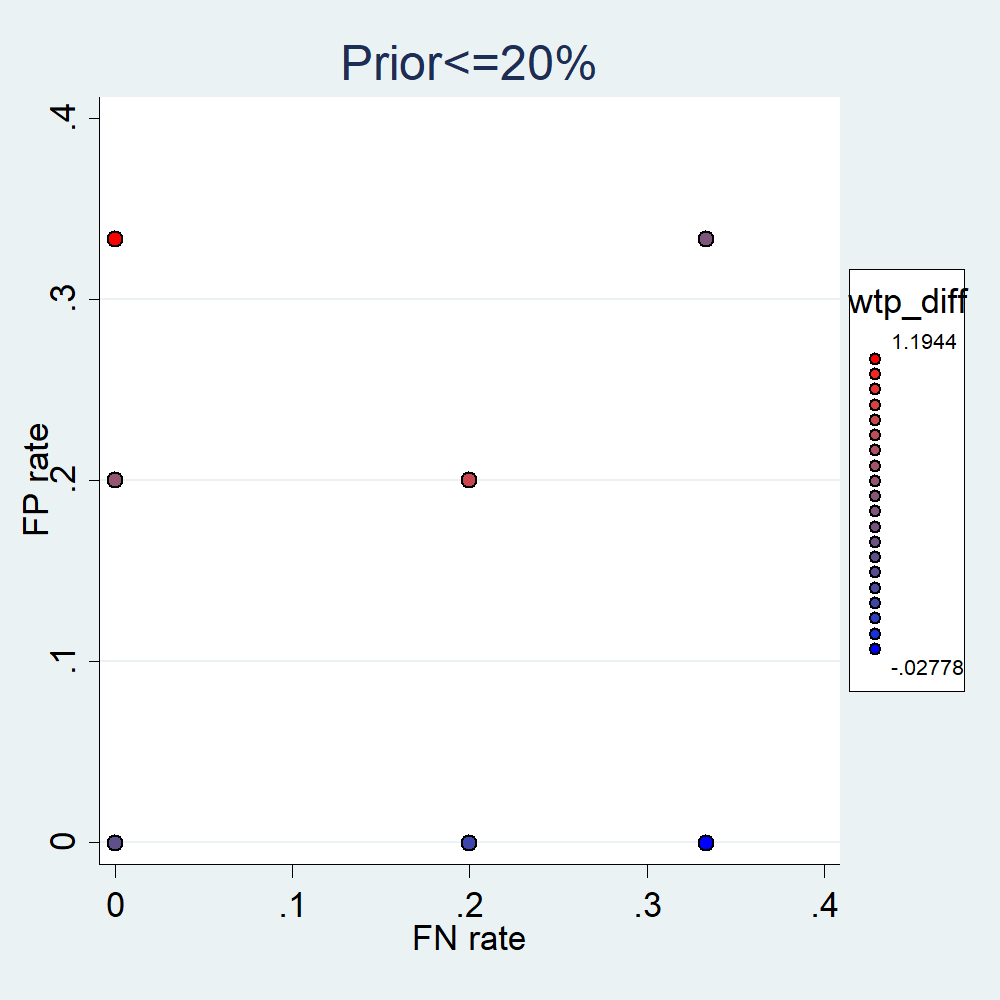
\includegraphics[width=\textwidth]{Graphs/WTP_pattern_low.png}
\end{subfigure}
~
\begin{subfigure}{0.5\textwidth}
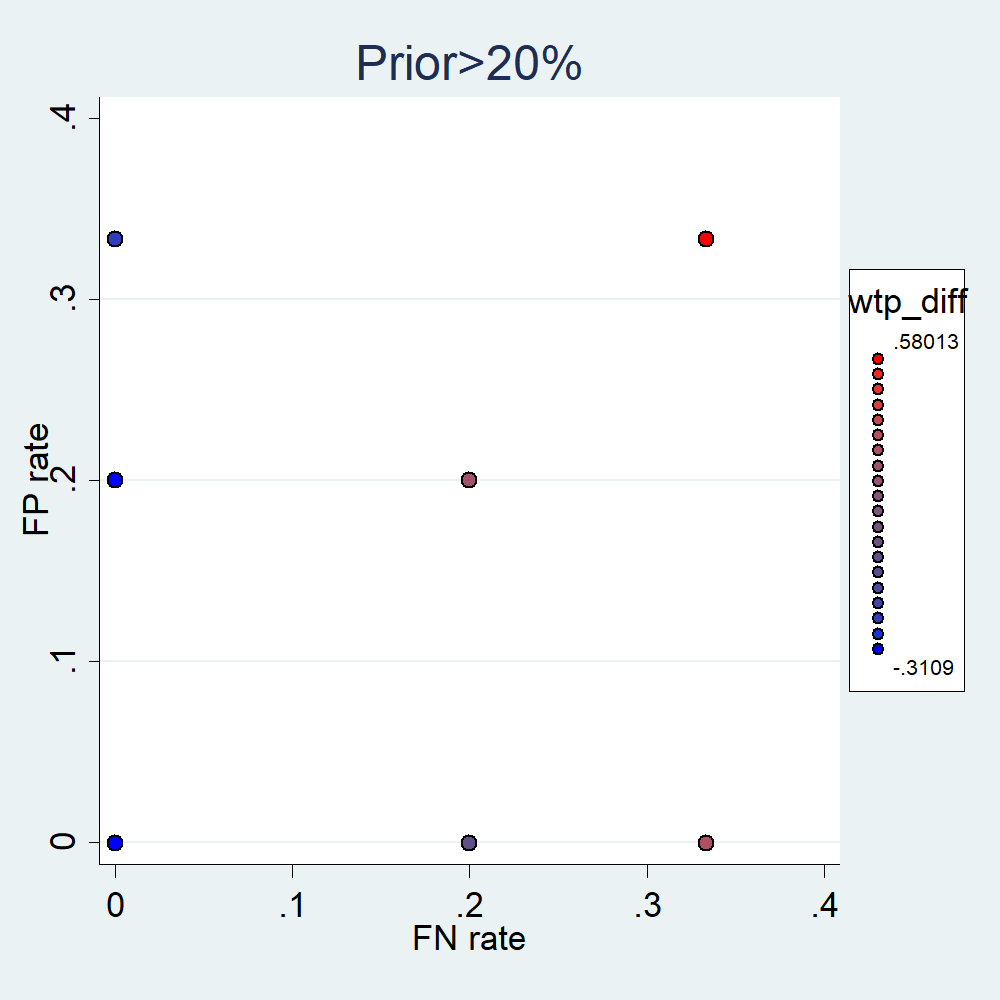
\includegraphics[width=\textwidth]{Graphs/WTP_pattern_high.png}
\end{subfigure}
\end{figure}
\end{frame}



\begin{frame}
\frametitle{Potential Explanations for the Heterogeneity}
\begin{enumerate}
\item Over-reacting to useless signals
\item Risk aversion with increasing third derivative (prudency)
\item Loss aversion
\item Probability weighting (part of cumulative prospect theory, rank-dependent EU, etc)
\item Probability estimation bias ("compounding neglect")
\end{enumerate}
\end{frame}


\begin{frame}
\frametitle{Potential Explanations: Reacting to Low-quality Signals}
\begin{itemize}
\item The signal's value for a risk-neutral agent is bounded below at zero: 
$$b^*=\max[0,\min(\pi L, c)-\pi P(s=0|\omega=1)L-P(s=1)c]$$
\item It is easy to prove that any signal with zero value $\pi P(s=0|\omega=1)L+P(s=1)c\leq \min(\pi L, c)$ generates either too low posterior probabilities to respond to any color or too high to not respond to any color
\item Potential issue: subjects are sensitive to signal's quality even for worthless signals
\end{itemize}
\end{frame}


\begin{frame}
\frametitle{Potential Explanations: Reacting to Low-quality Signals}
\begin{itemize}
\item Suppose that for given $\pi$ the theoretical value of the signal is non-positive $b^*\leq 0$
\item $\implies$ theoretical sensiivity to FP or FN is zero
\item If WTP sensitivity is non-zero (negative) - the difference has \textbf{negative} sensitivity
\item If the prior is low ($\pi L<c$) - most bad signals have high FP, so high negative sensitivity to FP
\item If the prior is high ($\pi L\geq c$) - most bad signals come from FN, so high negative sensitivity to FN
\item This prediction contradicts the observed pattern in which extra-negative sensitivity to FN emerges for low probs and vice versa 
\item Dropping obs with zero theoretical value or "forgetting" about bounds does not explain away the pattern
\end{itemize}
\end{frame}


\begin{frame}
\frametitle{Risk-averse decision-makers}
\begin{itemize}
\item Signal's value within EU framework is the maximum between 0 and the solution $b$ to the following equation:
$$P(S=B)u(Y-b-c)+\pi P(S=W|\omega=B)u(Y-b-L)+$$
$$+(1-\pi)P(S=W|\omega=W)=\pi u(Y-L)+(1-\pi) u(Y)$$
\begin{itemize}
\item where $P(S=W|\omega=B)$ - probability of having a negative signal (gremlin says white) conditional on the ball being black
\end{itemize}
\item What can be said about WTP? Not much:
\begin{itemize}
\item WTP can both increase and decrease with risk aversion even for honest treatments
\item Sensitivity to FP and FN can both increase and decrease depending on sign of $u'''()$
\end{itemize}
\end{itemize}
\end{frame}

\begin{frame}
\frametitle{Risk-averse decision-makers}

\begin{itemize}
\item Partial derivatives of WTP with respect to false-positive and false-negative rates:
\small
$${db\over dP(B|W)}=-{(1-\pi)(u(Y-b)-u(Y-c-b)\over D(\pi, P(W|B), P(B|W), b)}$$
$${db\over dP(W|B)}=-{\pi(u(Y-c-b)-u(Y-L-b)\over D(\pi, P(W|B), P(B|W), b)}$$
$$D(-)\equiv P(S=H)u'(Y-c-b)+\pi P(W|B)u'(Y-L-b)+$$
$$+(1-\pi)P(W|W)u'(Y-b)$$
\normalsize
\item Both sensitivities are negative, but we can't even say that sensitivities for str. concave $u()$ are higher or lower than risk-neutral sensitivities
\item The ratio of sensitivities: 
\small
$${db/dP(B|W)\over db/dP(W|B)}={(1-\pi)\over \pi} {u(Y-b)-u(Y-c-b)\over u(Y-c-b)-u(Y-L-b)}\leq {(1-\pi)\over \pi} {c\over L-c}$$
\end{itemize}
\end{frame}



\begin{frame}
\frametitle{Risk-averse decision-makers}
\begin{itemize}
\item For strictly concave $u()$ subjects  are relatively more sensitive to false-negative rates: $|db/dP(W|B)|>|db/dP(B|W)|$
\item What happens if we increase $\pi$? The first component is responsible for increasing sensitivity to false-negative rates, but there is also an effect of changing $b$...
\item In most (interesting) cases, WTP $b$ increases with priors $\pi$ shifting arguments of utility differences
\item Concavity $\implies$ difference in the numerator is "flatter", but concavity doesn't tell if the difference in flatness btw nominator and denominator goes up or down with $b$
\item When $u'''()>0$ (prudent) the ratio of utility differences goes up with $b$ and hence with $\pi$ $\implies$ underreacting to FN with growing $\pi$ as we observe
\end{itemize}
\end{frame}


\begin{frame}
\frametitle{Potential Explanations: Loss Aversion}
\begin{itemize}
\item Many potential framework for the loss aversion, but all assume that decision-makers have convex preferences in the loss domain
\item Empirically, loss aversion means overweighting small losses and underweighting large losses relative to small losses
\item It requires defining the loss domain and utility functions both for gains an the losses
\item Additionally, some loss aversion frameworks, including the common prospect theory also incorporate probability weighting
\item Consider Gul (1991) loss aversion framework:
$$V(X)=\sum p_k u(x_k)-\beta \sum p_k I(u(x_k)<\bar U)(\bar U-u(x_k))$$
\item Where $\bar U$ is the expected utility: $\bar U=\sum p_k u(x_k)$
\item Concave $u()$ $\implies$ $V()$ is convex in the loss domain
\end{itemize}
\end{frame}


\begin{frame}
\frametitle{Loss Aversion}
\begin{itemize}
\item Expected utility depends on priors, signal characteristics and utility function
\item $\implies$ Losses should include false negative outcomes (worst payoff), but also can include paying for protection
\item Theory has no say on whether the baseline should depend on no-protection option
\item For a given threshold it is indistinguishable from the EU framework (most likely, consistent with risk aversion)
\item Hence identification needs to rely on variation in the baseline outcome
\item If losses=false negative, then the ratio of sensitivities
\end{itemize}
\end{frame}





\begin{frame}
\frametitle{Loss Aversion}
\begin{itemize}
\item If losses=false negative, then the ratio of sensitivities:
\footnotesize
$${db/dP(B|W)\over db/dP(W|B)}={(1-\pi)\over \pi}{(1-\beta \pi P(W|B))(u(Y-b)-u(Y-c-b))\over D}$$
$$D=[\beta P(S=B)+(1-\beta \pi P(W|B)]u(Y-c-b)+(1-\pi)\beta(1-P(B|W))u(Y-b)+$$
$$+(2\beta \pi-1-\beta) u(Y-L-b)$$
\normalsize
\item Identical to the EU case with util. function $u()$ if $\beta=0$
\item Nominator is decreasing faster with $\pi$ compared to RN case
\item Denominator $D$ can both decrease and increase depending on $u()$ curvature and parameters chosen (likely to increase for our case)
\item Hence it is consistent with observed heterogen. response
\end{itemize}
\end{frame}


\begin{frame}
\frametitle{Loss Aversion: no Curvature case}
\begin{itemize}
\item If $u(x)=x$ and the loss domain includes the false-negative outcome only:
\small
$$b=BP_c - P(S=W)(1-\beta \pi P(W|B))c-\pi P(W|B)(1+\beta-\beta \pi P(W|B))L$$
$$BP_c \equiv \min[(1+\beta(1-\pi)\pi) L, c]$$
\normalsize
\item Sensitivity to false-positive rate decreases with $\pi$ relative to risk-neutral case:
\small
$${db \over dP(B|W)}=-(1-\pi)(1-\beta \pi P(W|B))c$$
\normalsize
\item The effect on false-negative rate is indeterminate (depends on signal quality, cost-loss ratio):
\small
$${db \over dP(W|B)}=-\pi((1+\beta-2\beta \pi P(L|H))L-(1-\beta(P(S=B)-\pi P(W|B)))c)$$
\normalsize
\end{itemize}
\end{frame}



\iffalse
\begin{frame}
\frametitle{Potential Explanations: Biased Belief Updating}
\begin{itemize}
\item A standard Bayesian agent does:
$$P(B|S)={P(S|B)P(B)\over P(S|W)P(W)+P(S|B)P(B)}$$
\item More generally, consider an agent updating as a quasi-Bayesian:
$$\mu(B|S)={P(S|B)^{\alpha}P(B){\beta}\over P(S|W)^{\alpha} P(W)^{\beta}+P(S|B)^{\alpha}P(B)^{\beta}} $$
\item You can estimate it as:
$$\log\left({\mu(B|S) \over 1-\mu(B|S)}\right)=\alpha \log\left({P(S|B) \over P(S|W)}\right)+\beta \log \left({P(B)\over P(W)}\right)$$
\item Base-rate neglect is when $0<\beta<1$ and $0<\alpha<1$ is the signal underweighting
\end{itemize}
\end{frame}


\begin{frame}
\frametitle{Belief Updating: Decomposition}
\footnotesize
\begin{table}[htbp]\centering
\def\sym#1{\ifmmode^{#1}\else\(^{#1}\)\fi}
\caption{Belief Elicitation: Decomposition}
\begin{tabular}{l*{3}{c}}
\hline\hline
                &\multicolumn{1}{c}{(1)}&\multicolumn{1}{c}{(2)}&\multicolumn{1}{c}{(3)}\\
                &\multicolumn{1}{c}{OLS}&\multicolumn{1}{c}{FE}&\multicolumn{1}{c}{Smart, FE}\\
\hline
lt\_prior        &     .178         &     .205\sym{**} &     .231\sym{**} \\
                &    (1.4)         &    (2.5)         &    (2.2)         \\
signalB         &   -.0835         &     .735\sym{**} &     .988\sym{**} \\
                &   (-0.2)         &    (2.5)         &    (2.5)         \\
signalW         &     .818\sym{***}&        0         &        0         \\
                &    (2.8)         &      (.)         &      (.)         \\
Constant        &     .332         &    -.471\sym{**} &    -.577\sym{**} \\
                &    (0.9)         &   (-2.7)         &   (-2.6)         \\
\hline
Observations    &       68         &       68         &       52         \\
Adjusted \(R^{2}\)&     0.16         &     0.20         &     0.25         \\
\hline\hline
\multicolumn{4}{l}{\footnotesize \textit{t} statistics in parentheses}\\
\multicolumn{4}{l}{\footnotesize \sym{*} \(p<0.10\), \sym{**} \(p<0.05\), \sym{***} \(p<0.01\)}\\
\end{tabular}
\end{table}

\end{frame}

\begin{frame}
\frametitle{Discussion: Belief Updating}
\begin{itemize}
\item Observe: base-rate neglect $\beta<0.3$ and the signal underweighting $0.3<\alpha<0.6$
\item Signal underweighting is much smaller
\item These findings are consistent with the meta-analysis in Benjamin (2018)
\item How does it affect WTP? 
\item Posterior probs do not enter the equation for the signal's value, but posteriors affect signal's responses
\item Approach: estimate posterior probs using the estimated quasi-bayesian equation above, find optimal responses and calculate the value of information for risk-neutral subject based on that $\rightarrow$ doesn't explain the pattern
\end{itemize}
\end{frame}



\begin{frame}
\frametitle{WTP difference: accounting for belief updating}
\footnotesize
{
\def\sym#1{\ifmmode^{#1}\else\(^{#1}\)\fi}
\begin{tabular}{l*{4}{c}}
\hline\hline
                &\multicolumn{1}{c}{(1)}&\multicolumn{1}{c}{(2)}&\multicolumn{1}{c}{(3)}&\multicolumn{1}{c}{(4)}\\
                &\multicolumn{1}{c}{0.1}&\multicolumn{1}{c}{0.2}&\multicolumn{1}{c}{0.3}&\multicolumn{1}{c}{0.5}\\
\hline
FP costs        &      .28\sym{*}  &    .0421         &    -.495\sym{**} &    -.547         \\
                &    (0.2)         &    (0.2)         &    (0.2)         &    (0.3)         \\
FN costs        &    .0622         &     1.55\sym{***}&     1.23\sym{***}&     .457\sym{***}\\
                &    (0.3)         &    (0.2)         &    (0.1)         &    (0.1)         \\
Constant        &     .467\sym{*}  &    -.359         &    -.605\sym{**} &     .811\sym{***}\\
                &    (0.2)         &    (0.2)         &    (0.3)         &    (0.3)         \\
\hline
Observations    &      162         &      153         &      162         &      153         \\
Adjusted \(R^{2}\)&     0.00         &     0.25         &     0.31         &     0.13         \\
\hline\hline
\multicolumn{5}{l}{\footnotesize Standard errors in parentheses}\\
\multicolumn{5}{l}{\footnotesize \sym{*} \(p<0.10\), \sym{**} \(p<0.05\), \sym{***} \(p<0.01\)}\\
\end{tabular}
}


\end{frame}
\fi

\begin{frame}
\frametitle{Alternative: Probability weighting}
\begin{itemize}
\item In EU framework subject weight outcome by their probabilities (or their beliefs)
\item In the prob. weighting framework the probabilities are rescaled towards the middle:
\item Tversky and Kahneman (1992) approach rescales probability $\mu$ into:
$$\phi(\mu)={\mu^{\gamma}\over [\mu^{\gamma}+(1-\mu)^\gamma]^{1/\gamma}}, 0<\gamma\leq 1$$
\item Difference: base-rate neglect affect only probabilities not given directly, probability weighting affects all the probabilities
\end{itemize}
\end{frame}


\begin{frame}
\frametitle{Probability weighting, risk-neutral case}
\begin{itemize}
\small
\item Use Tversky and Kahneman (1992):
$$b=\min[c,\phi(\pi) L]-\phi(P(S=B))c-\phi(\pi P(W|B))L$$
\item FP response:
$$db/dP(B|W)=-(1-\pi)\phi'(P(S=B))c$$
\item $\phi'(P(S=B))>1$ for small $P(S=B)$, but $\phi'(P(S=B))<1$ for larger $P(S=B)$
\item As $P(S=B)$ is increasing in $\pi$, sensitivity to FP rate decreases rel. to the baseline as $\pi$ grows (consistent with obs)
\item FN response:
$$db/dP(W|B)=-\pi (\phi'(\pi P(W|B))L-\phi'(P(S=B))c)$$
\item For $\pi P(W|B)<P(S=B)$ the sensitivity is higher than in RN case $|db/dP(W|B)|>\pi (L-c)$ but change of sensitivity with $\pi$ is unclear
\normalsize
\end{itemize}
\end{frame}


\begin{frame}
\frametitle{Probability Estimation Bias}
\begin{itemize}
\item Remember that WTP is:
\small
$$b=BP_c - P(S=W)(1-\beta \pi P(W|B))c-\pi P(W|B)(1+\beta-\beta \pi P(W|B))L$$
\normalsize
\item What if subjects do not correctly estimate the frequencies of FP $\pi P(B|W)$ and FN outcomes $(1-\pi)P(W|B)$?
\item Data: subjects do not increase (decrease) sensitivity to FN (FP) rates with increasing prior
\item It would explain the observed pattern
\item Similar but different from the base-rate neglect theory:
\begin{itemize}
\item Base-rate neglect: subjects underweight the base rate when calculating posterior probabilities
\item Here: subjects underweight the base rate when pricing signals (not accounting for growing impact of FN rates with increasing base rate)
\end{itemize}
\end{itemize}
\end{frame}



\begin{frame}
\frametitle{Comparative Analysis}
\footnotesize
\begin{table}[htbp]\centering
\begin{tabular}{l lc| c| c| c| c}
\hline \hline
\bf World & \multicolumn{2}{c}{\bf Low $\pi$} & \multicolumn{2}{c}{\bf High $\pi$} & \bf Ratio \\
\bf  & \bf FP& \bf FN & \bf FP & \bf FN &\bf FP/FN\\
\hline
\bf Observations & \bf $<$ & \bf $>$ & \bf $>=$ & \bf $<$ & \bf $\uparrow$ \\
\hline
Risk-averse and prudent & $><$ & $><$ & $><$ & $><$ & $\uparrow$ \\
Loss-averse &$<$ & $>$ & $><$ & $><$ & $><$\\
Probability-weighting & $>$ & $><$ &$<$ & $><$ & $><$ \\
Probability estimation bias & $<$ & $>$ &$>$ & $<$ & $\uparrow$ \\
\hline
\end{tabular}

\end{table}
\normalsize
\begin{itemize}
\item Can exclude probability-weighting explanation, but not loss aversion and risk aversion with prudence
\item Risk aversion explanation though depends on the curvature of $u()$ and the change of sensitivity with $\pi$ should be very small
\end{itemize}
\end{frame}


\begin{frame}
\frametitle{Comparative Analysis II}
\footnotesize
\begin{table}[htbp]\centering
\begin{tabular}{|llc|}
\hline \hline
\bf Model & \bf Prediction \\
\hline
Strict risk-aversion EU & Higher sensitivity to FN rates \\
\hline
Strict risk-aversion EU+prudence & \makecell[l]{Ratio of FN to FP \\sensitivities $\uparrow$ with $\pi$} \\
\hline
\multirow{2}{*}{Loss aversion} & FP sensit. $\downarrow$ with $\pi$ \\

 & FP sensit. is lower than for risk-neutral (RN) \\
\hline
\multirow{3}{*}{Probability weighting}  & \makecell[l]{FP sensit.$>$RN\\ for low $\pi$} \\

 & \makecell[l]{FP sensit.$<$RN \\for high $\pi$} \\

 & \makecell[l]{FN sensit. is higher  than RN \\for $\pi P(W|B)<P(S=B)<1/2$} \\
\hline
\multirow{3}{*}{Probability estimation bias}& \makecell[l]{FP sensitivity decreases \\with $\pi$ rel. to RN} \\
 & \makecell[l]{FN sensitivity increases \\with $\pi$ rel. to RN} \\
 & \makecell[l]{Diff. WTP for treatments \\with eq. FP and FN frequencies} \\
\hline

\end{tabular}

\end{table}
\end{frame}


\begin{frame}
\frametitle{Policy Implications: Probability Estimation Bias}
\begin{itemize}
\item Providing explicit probabilities of false positive and false negative outcomes should increase quality of decision-making (expected costs)
\item Providing explicit probabilities should increase WTP for high-quality alerts
\item Testable predictions:
\begin{itemize}
\item Signals with identical FP and FN frequencies but different priors and signal quality have different WTP (testing it in next slides)
\item Providing explicit probabilities should align WTP with the signal's value
\item With explicit probabilities subjects reduce their expected costs in the informed protection task
\end{itemize}
\end{itemize}
\end{frame}



\iffalse
\begin{frame}
\frametitle{Results: Probability weighting}
\begin{itemize}
\item Reweighting all the probabilities (blind protection included):
\end{itemize}
\footnotesize
{
\def\sym#1{\ifmmode^{#1}\else\(^{#1}\)\fi}
\begin{tabular}{l*{4}{c}}
\hline\hline
                &\multicolumn{1}{c}{(1)}&\multicolumn{1}{c}{(2)}&\multicolumn{1}{c}{(3)}&\multicolumn{1}{c}{(4)}\\
                &\multicolumn{1}{c}{0.1}&\multicolumn{1}{c}{0.2}&\multicolumn{1}{c}{0.3}&\multicolumn{1}{c}{0.5}\\
\hline
FP costs        &     .495\sym{***}&     .548\sym{***}&    -.198         &    -.275         \\
                &    (0.2)         &    (0.2)         &    (0.2)         &    (0.4)         \\
FN costs        &     1.65\sym{***}&     1.52\sym{***}&     1.04\sym{***}&     .535\sym{***}\\
                &    (0.2)         &    (0.1)         &    (0.1)         &    (0.1)         \\
Constant        &     -.77\sym{***}&     -1.2\sym{***}&    -.547\sym{**} &     .493\sym{*}  \\
                &    (0.2)         &    (0.2)         &    (0.2)         &    (0.3)         \\
\hline
Observations    &      162         &      153         &      162         &      153         \\
Adjusted \(R^{2}\)&     0.14         &     0.29         &     0.25         &     0.17         \\
\hline\hline
\multicolumn{5}{l}{\footnotesize Standard errors in parentheses}\\
\multicolumn{5}{l}{\footnotesize \sym{*} \(p<0.10\), \sym{**} \(p<0.05\), \sym{***} \(p<0.01\)}\\
\end{tabular}
}

\end{frame}


\begin{frame}
\frametitle{Results: Probability weighting}
\begin{itemize}
\item Reweighting only the probabilities not given directly (informed protection posterior probs but not blind protection):
\end{itemize}
\footnotesize
{
\def\sym#1{\ifmmode^{#1}\else\(^{#1}\)\fi}
\begin{tabular}{l*{4}{c}}
\hline\hline
                &\multicolumn{1}{c}{(1)}&\multicolumn{1}{c}{(2)}&\multicolumn{1}{c}{(3)}&\multicolumn{1}{c}{(4)}\\
                &\multicolumn{1}{c}{0.1}&\multicolumn{1}{c}{0.2}&\multicolumn{1}{c}{0.3}&\multicolumn{1}{c}{0.5}\\
\hline
FP costs        &     .418\sym{***}&     .656\sym{***}&      .72\sym{***}&     .694\sym{***}\\
                &    (0.0)         &    (0.0)         &    (0.0)         &    (0.1)         \\
FN costs        &      .94\sym{***}&     1.68\sym{***}&     1.53\sym{***}&     .817\sym{***}\\
                &    (0.1)         &    (0.1)         &    (0.0)         &    (0.0)         \\
Constant        &    -.799\sym{***}&    -2.36\sym{***}&    -3.08\sym{***}&    -2.56\sym{***}\\
                &    (0.0)         &    (0.0)         &    (0.0)         &    (0.0)         \\
\hline
Observations    &      162         &      153         &      162         &      153         \\
Adjusted \(R^{2}\)&     0.63         &     0.85         &     0.89         &     0.85         \\
\hline\hline
\multicolumn{5}{l}{\footnotesize Standard errors in parentheses}\\
\multicolumn{5}{l}{\footnotesize \sym{*} \(p<0.10\), \sym{**} \(p<0.05\), \sym{***} \(p<0.01\)}\\
\end{tabular}
}

\end{frame}
\fi


\begin{frame}
\frametitle{Accounting for Heterogeneity: Probability estimation bias}
\begin{itemize}
\item Next, test for the probability estimation bias
\item Does sensitivity to FP and FN varies with the base rate? No
\item Do priors, FP and FN rates affect WTP conditional on FP and FN frequencies (interactions)? Next table - yes.
\end{itemize}
\footnotesize
{
\def\sym#1{\ifmmode^{#1}\else\(^{#1}\)\fi}
\begin{tabular}{l*{4}{c}}
\hline\hline
                &\multicolumn{1}{c}{(1)}&\multicolumn{1}{c}{(2)}&\multicolumn{1}{c}{(3)}&\multicolumn{1}{c}{(4)}\\
                &\multicolumn{1}{c}{WTP}&\multicolumn{1}{c}{WTP(good quiz)}&\multicolumn{1}{c}{WTP(stateduc)}&\multicolumn{1}{c}{Value(RN)}\\
\hline
model           &                  &                  &                  &                  \\
p$>$0.2         &     1.02\sym{***}&     .918\sym{***}&     .999\sym{***}&     1.45\sym{***}\\
                &    (0.3)         &    (0.3)         &    (0.3)         &    (0.1)         \\
FP rate         &    -2.83\sym{**} &    -3.23\sym{**} &    -2.07         &    -4.74\sym{***}\\
                &    (1.1)         &    (1.4)         &    (1.3)         &    (0.3)         \\
p$>$0.2 $\times$ FP rate&    -.374         &    -.982         &    -.962         &     1.64\sym{***}\\
                &    (1.3)         &    (1.6)         &    (1.6)         &    (0.4)         \\
FN rate         &    -2.45\sym{**} &     -3.8\sym{***}&    -2.24\sym{*}  &    -1.74\sym{***}\\
                &    (1.1)         &    (1.3)         &    (1.3)         &    (0.3)         \\
p$>$0.2 $\times$ FN rate&    -.874         &    -.373         &    -.797         &    -3.12\sym{***}\\
                &    (1.3)         &    (1.5)         &    (1.6)         &    (0.4)         \\
Constant        &     1.72\sym{***}&     2.11\sym{***}&     1.56\sym{***}&     1.53\sym{***}\\
                &    (0.2)         &    (0.3)         &    (0.3)         &    (0.1)         \\
\hline
sigma           &                  &                  &                  &                  \\
Constant        &      1.9\sym{***}&     1.61\sym{***}&     1.82\sym{***}&     .495\sym{***}\\
                &    (0.1)         &    (0.1)         &    (0.1)         &    (0.0)         \\
\hline
Observations    &      630         &      342         &      378         &      630         \\
Adjusted \(R^{2}\)&                  &                  &                  &                  \\
\hline\hline
\multicolumn{5}{l}{\footnotesize Standard errors in parentheses}\\
\multicolumn{5}{l}{\footnotesize \sym{*} \(p<0.10\), \sym{**} \(p<0.05\), \sym{***} \(p<0.01\)}\\
\end{tabular}
}

\end{frame}



\begin{frame}
\frametitle{Accounting for Heterogeneity II: Probability estimation bias}

\footnotesize
{
\def\sym#1{\ifmmode^{#1}\else\(^{#1}\)\fi}
\begin{tabular}{l*{4}{c}}
\hline\hline
                &\multicolumn{1}{c}{(1)}&\multicolumn{1}{c}{(2)}&\multicolumn{1}{c}{(3)}&\multicolumn{1}{c}{(4)}\\
                &\multicolumn{1}{c}{}&\multicolumn{1}{c}{}&\multicolumn{1}{c}{}&\multicolumn{1}{c}{}\\
\hline
model           &                  &                  &                  &                  \\
FP rate         &    -4.34         &    -6.08\sym{*}  &    -4.62\sym{*}  &    -6.32\sym{*}  \\
                &    (2.8)         &    (3.3)         &    (2.8)         &    (3.3)         \\
FN rate         &    -2.38\sym{**} &    -.908         &    -2.71\sym{**} &    -1.32         \\
                &    (1.2)         &    (1.6)         &    (1.4)         &    (1.7)         \\
Stat. class     &                  &                  &    -.379         &    -.373         \\
                &                  &                  &    (0.2)         &    (0.2)         \\
Stat. class $\times$ FP rate&                  &                  &     .699         &     .645         \\
                &                  &                  &    (1.1)         &    (1.1)         \\
Stat. class $\times$ FN rate&                  &                  &     .524         &     .564         \\
                &                  &                  &    (1.1)         &    (1.1)         \\
Constant        &     1.54\sym{***}&     1.29\sym{***}&     1.79\sym{***}&     1.54\sym{***}\\
                &    (0.2)         &    (0.4)         &    (0.3)         &    (0.4)         \\
\hline
sigma           &                  &                  &                  &                  \\
Constant        &     1.86\sym{***}&     1.86\sym{***}&     1.85\sym{***}&     1.85\sym{***}\\
                &    (0.1)         &    (0.1)         &    (0.1)         &    (0.1)         \\
With squares    &       No         &      Yes         &       No         &      Yes         \\
\hline
Observations    &      624         &      624         &      624         &      624         \\
Adjusted \(R^{2}\)&                  &                  &                  &                  \\
\hline\hline
\multicolumn{5}{l}{\footnotesize Controlling for priors and total probabilities of false-posiive and false-negative outcomes. Standard errors in parentheses.}\\
\multicolumn{5}{l}{\footnotesize \sym{*} \(p<0.10\), \sym{**} \(p<0.05\), \sym{***} \(p<0.01\)}\\
\end{tabular}
}

\end{frame}


\end{document}

